\documentclass[english,10pt]{article}
\usepackage[utf8]{inputenc}
\usepackage[T1]{fontenc}
\usepackage{amsmath}
\usepackage{amssymb}
\usepackage{siunitx}
\sisetup{range-phrase={ -- }}
\sisetup{range-units=single}

\usepackage[english]{babel}
\usepackage{graphicx}
\graphicspath{{pics/}}
\usepackage[a4paper]{geometry}


\usepackage{verbatim}

\usepackage{xcolor}
\definecolor{link}{HTML}{4078C0}
\usepackage[colorlinks=true, allcolors = link]{hyperref}

\begin{document}
\begin{center}
\includegraphics[width = .3\textwidth]{page2_table1.png}
\end{center}
\setcounter{section}{4}
\setcounter{page}{2}
\section{Considerations Taken into Account for Device Sizing}

\paragraph{Sizing of $M_{n6}$}
${g_m}_{6}$ was chosen in order to bring $p_{2}$ further than $GBW$ so that $GBW$ is mainly determined by $p_1$.
${V_{ov}}_{6}$ was chosen very low based on output swing and power efficiency.
$L_{6}$ is chosen as long as possible in order to get good intrinsic gain and linearity. It is limited by $W_{6} < \SI{500}{\micro\meter}$ in order to limit parasitic capacitances. This limit is quickly reached since we need $g_m$ and weak inversion at the same time.
${V_{ds}}_6$ was chosen a bit higher than $\frac{V_{DD}}{2}$, to have almost symmetric swing and to get some more gain and linearity from the higher saturation.

\paragraph{Sizing of $M_{p5}$}
${i_{ds}}_5 = {i_{ds}}_6$.
${V_{ov}}_5$ was chosen low based on the output swing.
${V_{ds}}_5 = {V_{ds}}_6 - V_{DD}$.
$L_{5}$ was chosen very long to have a current source as ideal as possible. To ensure matching and linearity, every transistor in the current mirror should have the same length. $L_{5}$ is thus limited by the width and the parasitic capacitances of any of ${M_p}_{5}, \: {M_p}_{7}, \: {M_p}_{8}$.

\paragraph{Sizing of ${M_p}_{1},\:{M_p}_2$}
Those transistors should have the same sizing and biasing so that the pair is symmetric.
${g_m}$ is chosen based on $f_{GBW}$.
$V_{ov}$ is chosen low based on power efficiency.
${V_{db}} = {V_{gs}}_6$.
$V_{gb}$ was chosen so that $|V_{ds}| > |V_{dsat}| \simeq |V_{ov}|$.
$L$ was chosen as long as possible to maximize intrinsic gain and linearity. It is limited by $W$. The same consideration as for ${M_p}_6$ stands.

\paragraph{Sizing of ${M_{n}}_3, \:{M_{n}}_4$}
Those transistors should have the same sizing and biasing so that the pair is symmetric.
${i_{ds}} = {i_{ds}}_1 = {i_{ds}}_2$.
${V_{ds}} = {V_{gs}} = {V_{gs}}_6$.
$L$ was chosen very long to minimize $g_{ds}$ and maximize linearity.

\paragraph{Sizing of ${M_{p}}_7$}
${i_{ds}}_7 = 2 {i_{ds}}_1$.
$L_7 = L_5$ to reduce distortion within the current mirror. $L$ was chosen long to have current sources as ideal as possible.
${V_{gs}}_7 = {V_{gs}}_5$.
${V_{ds}}_7 = {V_{sb}}_2$.

\paragraph{Sizing of ${M_{p}}_8$}
${V_{gs}}_8 = {V_{ds}}_8 = {V_{gs}}_5 = {V_{gs}}_7$.
$L_8 = L_7 = L_5$ to reduce distortion within the current mirrors.
${i_{ds}}_8$ was chosen 100 times smaller than the smallest stage current, because ${M_{p}}_8$ should not contribute to the power consumption, since ${i_{ds}}_8$ is wasted current.

\paragraph{Sizing of $C_{m}$}
$C_{m}$ was chosen 5 -- 10 times smaller than $C_L$ so that the Miller pole is the dominant one. On the one hand, a too large Miller capacitance would load much the first stage too much to meet the spec on $GBW$. On the other hand, a too small Miller capacitance would load the transistor $M_{n6}$ too much in order to meet the spec on $A_v$, if the spec on $GBW$ is strictly respected.

\paragraph{Sizing of $R_{m}$}
The nulling Miller resistance was chosen in order to cancel the second pole of the OTA and thus increase its phase margin.

\section{Simulation Results}
\subsection{Frequency Response}
\subsubsection{Final Design}\label{sec:final}
\begin{figure}[htbp]
  \centering
  \includegraphics[width = \textwidth]{6_1.pdf}
  \caption{Bodeplots: final design\label{fig:final}}
\end{figure}
Figure \ref{fig:final} shows the bodeplots of the final OTA, as simulated by Matlab and Spectre. We observe that the matlab simulation was mostly accurate and that the design, as simulated Spectre seems to meet all the specs. We see however that Spectre shows that the miller zero is a bit slower than the second stage pole, and that the next pole is a bit slower than predicted. This appears mostly on the phase graph, where we see that the phase rises up a bit after the first pole, rather than staying flat. The phase then starts to decrease again a bit before what was predicted using Matlab.

On figure \ref{fig:final}, we read a phase margin of \SI{90.78}{\degree} as per Spectre and of \SI{83.8}{\degree} as per Matlab.

\subsubsection{Effect of the Compensation Network}
\begin{figure}[htbp]
  \centering
  \includegraphics[width = \textwidth]{6_2.pdf}
  \caption{Bodeplots: effect of the compensation network\label{fig:comp}}
\end{figure}
Figure \ref{fig:comp} shows the effect of the compensation network. With no compensation, we see that the OTA becomes externally compensated: the dominant pole is set by the output node and depends on $C_L$. This increases $f_{GBW}$ but degrades the phase margin a lot, since the next poles as we can see on the phase graph, follow nearly immediately. The phase margin is reduced to \SI{0.62}{\degree} as per Spectre and to \SI{2.88}{\degree} as per Matlab. The bode curves differ between Matlab and Spectre, which is expected since parts of the Matlab simulation rely on the OTA being internally compensated.

With only the Miller capacitor, we see that the OTA becomes internally compensated, and the bodeplot before $f = \SI{2}{\mega\hertz}$ is satisfyingly shaped. However, the lack of nulling resistor means it is not possible to cancel the second pole in order to increase the phase margin and the bandwidth in which the OTA behaves as a first order circuit. The phase margin is \SI{51.5}{\degree} as per Spectre and \SI{44.1}{\degree} as per Matlab.

With bot the compensation capacitor and the compensation resistor, we come back on our final design, which is analysed in \ref{sec:final}.

\subsubsection{Effect of the Load Capacitance}
Figure \ref{fig:cl}
\begin{figure}[htbp]
  \centering
  \includegraphics[width = \textwidth]{6_3.pdf}
  \caption{Bodeplot: effect of the load capacitance\label{fig:cl}}
\end{figure}
shows the effect of the load capacitance $C_L$. We see that it doesn't affect the frequency response before \SIrange{2}{4}{\mega\hertz}, which is normal since it doesn't appear in the DC gain, and since the OTA is internally compensated. With every parameter of the OTA fixed, decreasing $C_L$ makes the second stage pole faster\footnote{In first approximation, we have $p_1 = \frac{{g_m}_6}{C_L}$}, which improves the high frequency response: the gain decreases slower and the phase margin is higher: \SI{107.3}{\degree} as per Spectre and \SI{85.4}{\degree} as per Matlab. Since the miller zero does not move, its effect becomes very clear when the second stage pole is brought to higher frequencies.

Conversely, increasing $C_L$ makes the second stage pole slower, which degrades the high frequency response: the gain decreases faster and the phase margin is lower: \SI{80.0}{\degree} as per Spectre and \SI{82.2}{\degree} as per Matlab.

In conclusion, we see that, as expected, the OTA works better as the load input impedance is closer to ideal, or in terms of transistor characteristics, as the next stage has lower parasitic capacitances. However, we also see that since the OTA is internally compensated, its frequency response is not impacted too much at the end of the day by a \SI{50}{\percent} change on the load, which is a real advantage.

\subsubsection{Effect of the Miller Capacitance}
Figure~\ref{fig:cm}
\begin{figure}[htbp]
  \centering
  \includegraphics[width = \textwidth]{6_4.pdf}
  \caption{Bodeplots: Effect of the Miller Capacitance\label{fig:cm}}
\end{figure}
shows the effect of the Miller capacitance $C_m$. We see that it directly affects the $f_GBW$ which is expected since decreasing $C_m$ brings the dominant pole to higher frequencies\footnote{In first approximation, we have $p_2 = \frac{{g_m}_2}{C_m}$}. However, since the second stage pole is then left unchanged $\frac{p_1}{p_2}$ is reduced, and this leads to a degradation of the phase margin. With $C_m = \SI{8}{\pico\farad}$, the phase margin is \SI{83.7}{\degree} as per Spectre and \SI{81.2}{\degree} as per Matlab.

Conversely, increasing $C_m$ reduces $f_GBW$ and increases the phase margin: for $C_m = \SI{12}{\pico\farad}$, the phase margin is \SI{96.7}{\degree} as per Spectre and \SI{85.3}{\degree} as per Matlab. The effect of $C_m$ is pretty direct to predict.

\subsection{Noise and Large Signal Distortion}
\subsubsection{Input Noise Voltage}
Figure~\ref{fig:noise}
\begin{figure}[htbp]
  \centering
  \includegraphics[width = \textwidth]{noise_1.pdf}
  \caption{Input referred voltage noise power spectral density\label{fig:noise}}
\end{figure}
shows the input referred voltage noise power spectral density from \SI{1}{\hertz} to \SI{100}{\giga\hertz}. The shape is easy to predict up to \SI{10}{\giga\hertz}: if we consider a second order circuit affected by pink output noise, this shape is produced when the turning point is between the first and second poles of the circuit. This is shown on the asymptotic magnitude plot of figure \ref{fig:noiseAsym}.
\begin{figure}[htbp]
  \centering
  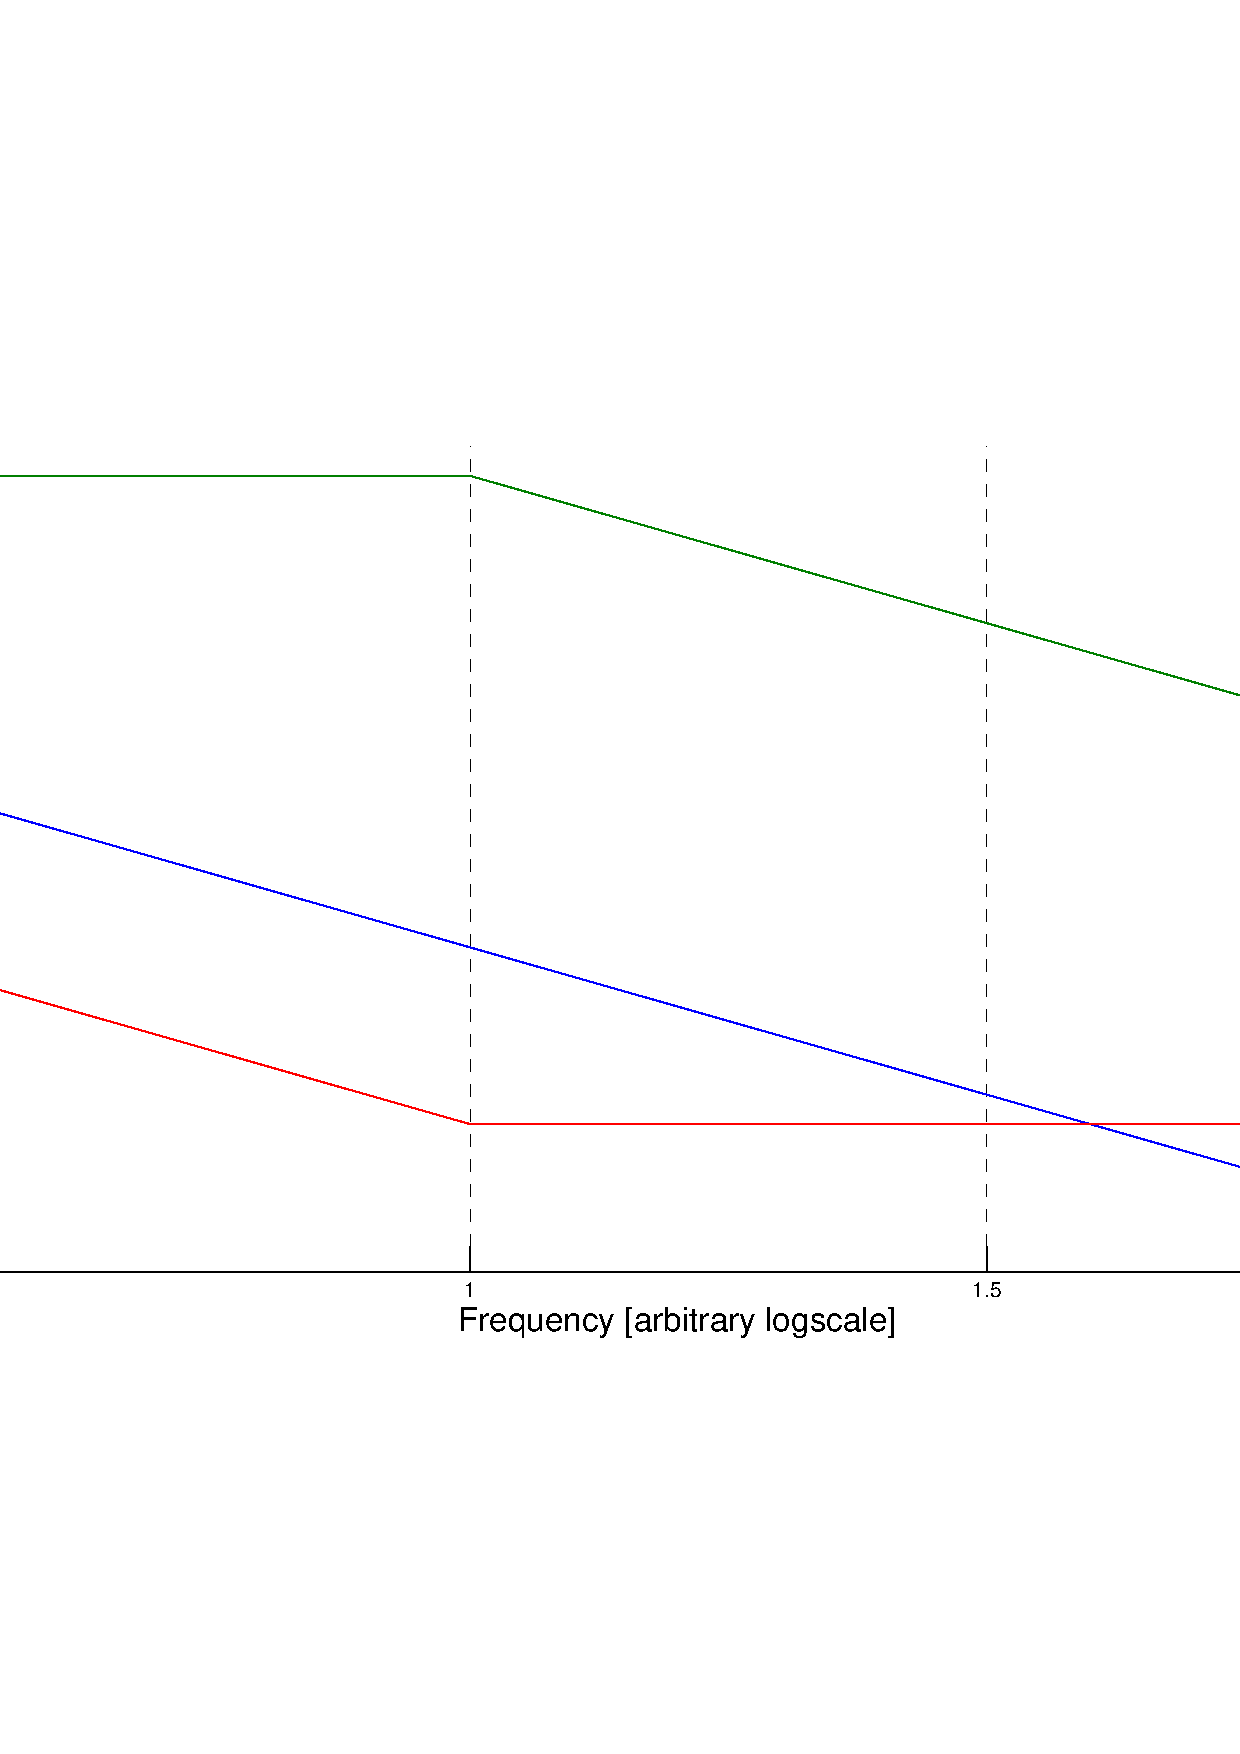
\includegraphics[width = \textwidth]{noiseAsym.pdf}
  \caption{Asymptotic magnitude plot predicting the noise density shape (arbitrarily scaled)\label{fig:noiseAsym}}
\end{figure}
The input noise dip at around \SI{10}{\giga\hertz} is most probably due to higher order zeroes in the OTA as well as inaccuracies in the solver for such high frequencies.

\subsubsection{Total Input Referred Noise Voltage}
Table~\ref{tab:noise}
\begin{table}[htbp]
  \centering
  \begin{minipage}{10cm}
  \verbatiminput{noise_2.dat}
  \caption{Noise summary of the final OTA\label{tab:noise}}
  \end{minipage}
\end{table}
shows the noise summary of the OTA and the top 10 contributors to the input voltage noise power integrated from \SI{1}{\hertz} to \SI{100}{\giga\hertz}. We see that, as expected, the noise from the input stage is the dominant factor. The $^1/_f$ seems to dominate the over white noise.

\subsubsection{Large Signal Distortion}
Figure~\ref{fig:large}
\begin{figure}[htbp]
  \centering
  \includegraphics[width = \textwidth]{noise_3.pdf}
  \caption{Large signal operation of the final OTA\label{fig:large}}
\end{figure}
shows the voltage gain and the output voltage as a function of the input signal amplitude. On the output voltage curve, we see that the operation is linear up until approximately \SI{1}{\milli\volt}. We then observe significant distortion, until the output stage leaves saturation, at which point the output voltage is nearly unchanged by an increase in input voltage.

The voltage gain curve shows similar information. We read 1-dB compression point of \SI{1.18}{\milli\volt}.
\end{document}
